\documentclass[notes]{beamer}
\usepackage{hyperref}
\usepackage{graphicx}
\mode<article>
    {
      \usepackage{fullpage}
      \usepackage{pdf}
      \usepackage{hyperref}
    }
    
\mode<presentation>{
  \usetheme{Dresden}
  \setbeamercovered{transparent}
}

\title{HacDC}
\author{Serge Wroclawski}
\begin{document}
\section{The Objective}

\begin{frame}
  \frametitle{What is HacDC?}
  From \href{http://www.hacdc.org}{hacdc.org}:
  \begin{quote}
    HacDC is a non-profit organization and space dedicated to
    technical, artistic and social collaboration. We are
    technologists, tinkerers, crafters and codemonkeys who call DC
    home. We collaborate across disciplines for the benefit of
    cultural, charitable and scientific causes. We create, learn and
    teach as a group, inviting our neighbors around the block and
    around the world to join us.
  \end{quote}
\end{frame}

\begin{frame}
  \frametitle{Does HacDC Do?}
  \begin{itemize}
  \item Provides a workshop for people to work on ongoing projects
  \item New Workshop Coming Soon!
  \item Provides a meeting space for groups
  \item An organization to bring communities together
  \end{itemize}
\end{frame}

\begin{frame}
  \frametitle{Does HacDC Do?}
  \begin{itemize}
  \item Provides a workshop for people to work on ongoing projects
    \uncover<3>{
      \begin{itemize}
      \item Lots of free parts of every sort (motors, cables, raw materials)
      \item A stocked pantry of low-cost parts (IC chips, microcontrollers, LEDs)
      \item Free supplemental parts (solder, wire)
      \item Lots of tools!
      \end{itemize}
    }
  \item New Workshop Coming Soon!
    \uncover<4>{
      \begin{itemize}
      \item New Workshop being built in basement
      \item Will allow for larger projects (possible wood or metal-working)
      \end{itemize}
    }
  \item Provides a meeting space for groups
    \uncover<5>{
      \begin{itemize}
      \item The Workshop, Church Auditorium, Church Dining Room
      \end{itemize}
    }
  \item An organization to bring communities together
    \uncover<6>{
      \begin{itemize}
      \item Software People
      \item Hardware People
      \item Artists
      \end{itemize}
    }
  \end{itemize}
\end{frame}

\section{The Space}

\begin{frame}[fragile]
  \frametitle{The Space!}
  \begin{center}
    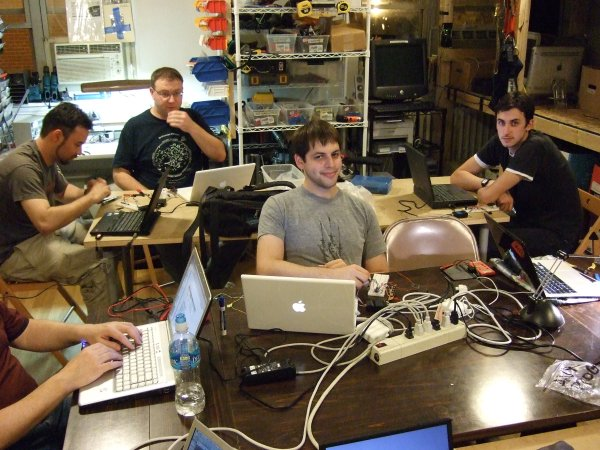
\includegraphics[width=.8\textwidth,height=.8\textheight]{dscf2730_small.jpg} \\
    {\em A classroom full of people on Microcontroller Mondays.}
  \end{center}
\end{frame}

\begin{frame}
  \frametitle{The Significance of the Space}
  \begin{itemize}
  \item The main differiantor between HacDC and other groups
  \item Teaching Space
  \item Workshop
  \item Social Space
  \item Open 24/7
  \end{itemize}
\end{frame}

\section{The Activities}

\begin{frame}
  \frametitle{HacDC Activities}
  \begin{itemize}
  \item Classes
    \begin{itemize}
    \item Microcontroller Class
    \item Electronics Class
    \item Programming Classes (C, C++, Ruby)
    \end{itemize}
  \item Weekly Talks
    \begin{itemize}
    \item Lasers
    \item Art Hacking
    \item Community Building
    \end{itemize}
  \item Group Meetings/Project Gatherings
    \begin{itemize}
    \item Clojure Study Group
    \item Multi-Touch Display
    \end{itemize}
  \item Special Events
    \begin{itemize}
    \item Electronics with Mitch Altman
    \item RepRap Build-A-Thon
    \end{itemize}
  \item Social Gatherings
   
   \begin{itemize}
   \item Movie Nights
   \item SchmooCon Party, DCLinuxChix Party
   \end{itemize}
  \end{itemize}
\end{frame}

\section{Future Plans}

\begin{frame}
  \frametitle{Future Plans}
  \begin{itemize}
  \item More Classes
  \item More Special Events
  \item More Community Service
  \end{itemize}
\end{frame}

\section{Getting Involved}

\begin{frame}
  \frametitle{Getting Involved}
  \begin{itemize}
  \item Go to \href{http://hacdc.org}{hacdc.org}
    \begin{itemize}
    \item Check out the blog
    \item Check out the calendar
    \item Get on the announce or blabber lists
    \end{itemize}
  \item Go to our events
    \begin{itemize}
    \item They're all free and open to the public
    \end{itemize}
  \item Become a member
    \begin{itemize}
    \item Access to the workshop
    \item Hold meetings
    \item Help shape the organization
    \end{itemize}
  \end{itemize}
\end{frame}

\section{Questions}

\begin{frame}
  \begin{center}
    {\Large Questions?}
  \end{center}
\end{frame}

\section{Thanks and License}

\begin{frame}
  Special Thanks to:
  Tim Collins, Mitch Altman and Elliot Williams for the great photographs
  
  To DCLUG for providing me a forum for more than twelve years.
  And to HacDC for inspiration for this talk.
  
  Copyright \copyright 2009 Serge Wroclawski <serge@wroclawski.org>
  
  This presentation is available under the Creative Commons
  Attribution-ShareAlike License.
  
  Current versions of this presentation are available at:
  
\end{frame}

\end{document}